\documentclass[10pt, oneside]{article}

\input ./combined_macros.sty

\addbibresource{Twist.bib}

\usepackage{pdflscape}
\usetikzlibrary{shapes.geometric, arrows, positioning}

\tikzstyle{s16} = [rectangle, rounded corners, minimum width=2cm, minimum height=1cm,text centered, draw=black,fill=red!30]
\tikzstyle{s16chiral} = [s16, dashed]
\tikzstyle{s8} = [rectangle, rounded corners, minimum width=2cm, minimum height=1cm,text centered, draw=black,fill=orange!30]
\tikzstyle{s4} = [rectangle, rounded corners, minimum width=2cm, minimum height=1cm,text centered, draw=black,fill=yellow!30]
\tikzstyle{s2chiral} = [rectangle, dashed, rounded corners, minimum width=2cm, minimum height=1cm,text centered, draw=black,fill=green!30]
\tikzstyle{dimension} = [ellipse, text centered, text width=1cm, minimum height=1cm, draw=black]
\tikzstyle{arrow} = [thick,->,>=stealth]

\title{Twists of supersymmetric gauge theories}
\author{Chris Elliott\and Pavel Safronov \and Brian Williams}

\date{\today}

\begin{document}

\maketitle

\section*{Introduction}

\section{Preliminaries}

Throughout the paper we will mostly work with a $\ZZ\times\ZZ/2$-grading. \emph{Degree} will refer to the first (cohomological) grading and \emph{odd} or \emph{even} to the second (fermionic) grading.

\subsection{The definition of a field theory}

\begin{dfn}
A {\bf free BV theory} on a manifold $M$ is the data:
\begin{itemize}
\item a finite rank $\ZZ\times\ZZ/2$-graded vector bundle $E \to M$ equipped with an even differential operator of cohomological degree $+1$
\[
Q \colon \cE \to \cE [1] 
\]
such that $(1)$: $Q^2 = 0$ and $(2)$: the pair $(\cE , Q)$ is an elliptic complex;
\item a map of bundles
\[
\omega\colon E \otimes E \to {\rm Dens}_M [-1]
\]
that is
\begin{enumerate}
\item[$(1)$] fiberwise nondegenerate,
\item[$(2)$] graded skew symmetric, and
\item[$(3)$] satisfies $\int_M \omega\<e_0, Q e_1\> = (-1)^{|e_0|} \int_M \omega(Q e_0, e_1)$ where $e_i$ are compactly supported sections of $E$ .
\end{enumerate}
\end{itemize}
\end{dfn}

\brian{recall dfn of $\oloc$ of a gr vb.}

\begin{dfn}
A {\bf classical BV field theory} (or simply, classical field theory) is a free BV theory $(E, Q, \omega)$ equipped with an even functional
\[
I \in \oloc^+(E)
\]
of cohomological degree zero satisfying the classical master equation 
\[
Q I + \frac{1}{2} \{I,I\} = 0 .
\]
\end{dfn}

Given a classical field theory $(E, Q, \omega, I)$ we denote by
\[S = \frac{1}{2} \int_M \omega(e, Q e) + I\in \oloc(E)\]
the BV action of the theory.

\begin{remark}
We will also consider $\ZZ/2$-graded classical field theories which are defined as before, but where $E$ has only a single $\ZZ/2$-grading and, correspondigly, $Q$ is simply an odd operator.
\end{remark}

A local functional induces an endomorphism $\{I,-\}$ on the space of all local functionals $\oloc(E)$. 
It also induces an endomorphism on the larger space of {\em all} functionals $\cO(E)$. 
The classical master equation implies that the operator $Q + \{I,-\}$ squares to zero on $\cO(E)$, and hence every classical field theory defines a cochain complex
\[
\left(\cO(E), Q + \{I,-\}\right) .
\]
We will refer to this as the {\bf classical BV complex} of the theory. 

\begin{dfn}
A {\bf morphism} of classical field theories (defined on the same manifold $M$) $F\colon (E, Q, \omega, I) \to (E', Q', \omega', I')$ is a linear map of vector bundles
\[
F\colon E \to E'
\]
that intertwines the differentials $Q, Q'$, the pairings $\omega, \omega'$, and the interactions $I,I'$. 
\end{dfn}

Note that a map of classical field theories induces a map of BV complexes
\[
F^*\colon \left(\cO (\cE)[-1], Q + \{I,-\} \right) \to \left(\cO (\cE')[-1], Q' + \{I',-\} \right) .
\]
This allows us to make the following definition of an equivalence between classical theories. 

\begin{dfn} \label{equivalence_def}
A morphism of classical field theories $F\colon (E, Q, \omega, I) \to (E', Q', \omega', I')$ is an {\bf equivalence} if it induces a quasi-isomorphism 
\[
F^* \colon  \left(\cO(\cE')[-1], Q' + \{I',-\} \right) \xto{\simeq} \left(\cO(\cE)[-1], Q + \{I,-\} \right) .
\]
\end{dfn}

\begin{dfn}
Let $(E, Q,\omega, I)$ be a classical field theory 
A {\bf strict action} of a super Lie algebra $\fg$ on $(E, Q,\omega, I)$ is a map of super dg Lie algebras
\[
\rho\colon \fg \to \left(\oloc(E)[-1] , \{-,-\}_\omega, Q + \{I,-\}_\omega\right) .
\]
More generally, an $L_\infty$ {\bf action} is an $\infty$-morphism of super dg Lie algebras
\[
\rho\colon \fg \rightsquigarrow \left(\oloc(E)[-1] , \{-,-\}_\omega, Q + \{I,-\}_\omega\right) .
\]
\brian{maybe point to appendix where we can fix conventions for $\infty$-maps}
\end{dfn}

We denote components of an $\infty$-morphism by $\rho_2, \rho_3, \dots$, so that $\rho_2$ is a morphism of (super) chain complexes.

\subsection{The classical factorization algebra}

\pavel{explain how to obtain a factorization algebra from a classical field theory.}

Let $(E, Q, \omega, I)$ be a classical field theory and suppose $\psi_0 \in \sE$ is a fixed solution to the equations of motion. 
Then, we recall the formalism of \cite{CG1,CG2} which extracts a factorization algebra on spacetime that should be thought of as  functions on the formal neighborhood of the derived critical locus of the action $S$ near $\psi_0$. 

\begin{dfn}
Let $(E, Q, \omega, I)$ be a classical field theory on $M$.
The {\bf classical factorization algebra of observables} $\Obs$ assigns to an open set $U \subset M$ the commutative dg algebra
\[
\Obs(U) = \left(\cO(\cE(U)) , Q + \{I,-\}\right) .
\]
\end{dfn}

\subsection{From BRST to BV}


\pavel{explain how to get a BV theory from a BRST theory}

%\begin{dfn}
%A {\bf classical BRST theory} is a finite rank $\ZZ \times \ZZ / 2$-graded vector bundle $F \to M$ equipped with an even differential operator of cohomological degree $+1$
%\[
%Q : \cF \to \cF[1]
%\]
%such that $Q

\subsection{Examples}

\pavel{(partially) topological BF theories and Chern-Simons theories in different dimensions.}

\subsection{Supersymmetry} \label{sec: susy}

In this section we recall the framework for supersymmetry following \cite{ElliottSafronov} and \cite{DeligneSpinors}, we refer there for more details.

Let $V_\RR = \RR^n$ endowed with its nondegenerate bilinear form and $V=V_\RR\otimes_\RR\CC$ its complexification. Consider the Lie algebra $\so(V)$. Let us recall the following facts:
\begin{itemize}
\item If $n$ is odd, $\so(V)$ has a distinguished fundamental representation called the {\bf spin} representation $S$.

\item If $n$ is even, $\so(V)$ has a pair of distinguished fundamental representations called the {\bf semi-spin} representations $S_+, S_-$.
\end{itemize}

\begin{dfn}
A {\bf spinorial representation} $\Sigma$ is a sum of spin or semi-spin representations of $\so(V)$.
\end{dfn}

So, in odd dimensions we have $\Sigma=S\otimes W$ and in even dimensions we have $\Sigma=S_+\otimes W_+\oplus S_-\otimes W_-$, where $W$ denotes a multiplicity space.

\begin{dfn}
Fix a spinorial representation $\Sigma$ and a nondegenerate $\so(V)$-equivariant pairing $\Gamma\colon \sym^2(\Sigma)\rightarrow V$. The {\bf supertranslation Lie algebra} is the $\so(V)$-equivariant super Lie algebra $T=\Pi\Sigma\oplus V$ whose only nontrivial bracket is given by $\Gamma$.
\end{dfn}

For a given spinorial representation, the pairing $\Gamma$ is unique up to a scale, so a supertranslation Lie algebra is specified by fixing a spinorial representation. In turn, a spinorial representation is determined by the dimension of the multiplicity space, so we will talk about $\mc{N}$ or $(\mc{N}_+, \mc{N}_-)$ supertranslation Lie algebras, where the numbers are specified as follows:
\begin{itemize}
\item If $n\equiv 0, 1, 3, 4\pmod 8$, we let $\mc{N} = \dim(W)$.

\item If $n\equiv 2 \pmod 8$, we let $\mc{N}_{\pm}=\dim(W_{\pm})$.

\item If $n\equiv 5, 7\pmod 8$, we let $2\mc{N} = \dim(W)$.

\item If $n\equiv 6\pmod 8$, we let $2\mc{N}_{\pm} = \dim(W_{\pm})$.
\end{itemize}

Fix the following data:
\begin{itemize}
\item A spinorial representation $\Sigma$ of $\so(V)$.

\item An $\so(V)$-equivariant nondegenerate pairing $\Gamma\colon \sym^2(\Sigma)\rightarrow V$.

\item A complex Lie group $G_R$, the {\bf group of $R$-symmetries}, which is a subgroup of $\so(V)$-equivariant automorphisms of $(\Sigma, \Gamma)$.
\end{itemize}

Note that the supertranslation Lie algebra $T$ is a $\Spin(V_\RR)\times G_R$-equivariant super Lie algebra.

Consider a spacetime manifold $M$ which is an affine space over $V_\RR$. Let $\ISO(V_\RR) = \Spin(V_\RR)\ltimes V_\RR$ be the Poincar\'{e} group which acts in the obvious way on $M$.

\begin{dfn}
A classical field theory $(E, Q, \omega, I)$ is {\bf supersymmetric} if $E\rightarrow M$ is an $\ISO(V_\RR)\times G_R$-equivariant vector bundle and the infinitesimal strict action of the translation Lie algebra $V$ on the classical theory is extended to a $\Spin(V_\RR)\times G_R$-equivariant $L_\infty$ action of the supertranslation Lie algebra $T$ on the classical theory.
\end{dfn}

\subsection{Supersymmetric twisting}

\begin{dfn}
A {\bf square-zero supercharge} is a nonzero element $Q\in\Sigma$ such that $\Gamma(Q, Q)=0$.
\end{dfn}

It is shown in \cite[Proposition 3.25]{ElliottSafronov} that the image of $\Gamma(Q, -)\colon \Sigma\rightarrow V$ has dimension at least $n/2$. We will use the following adjectives for square-zero supercharges depending on $d=\dim(\mathrm{im}\Gamma(Q, -))$:
\begin{itemize}
\item A supercharge $Q$ is {\bf topological} if $d = n$.

\item A supercharge $Q$ is {\bf holomorphic} if $n$ is even and $d=n/2$.
\end{itemize}

In the intermediate case we refer to $Q$ as a {\bf holomorphic-topological} (alternatively, partially topological) supercharge. The collection of all square-zero supercharges in dimensions 2 through 10 (where one restricts to supersymmetries with at most 16 supercharges) was studied in \cite{ElliottSafronov} and \cite{EagerSaberiWalcher}. In particular, orbits of square-zero supercharges under the $R$-symmetry group, $\Spin(V)$ and the obvious scaling action of $\CC^\times$ are shown in Figure \ref{fig:superchargeorbits}:
\begin{itemize}
\item The color denotes the amount of supersymmetries: red denotes 16 supercharges, orange 8 supercharges, yellow 4 supercharges and green 2 supercharges. Dashed border denotes chiral supersymmetry (i.e. $(\cN_+, 0)$ in even dimensions).

\item $d$ denotes the dimension of the image of $\Gamma(Q, -)$.

\item Rank denotes the rank of the tensor $Q\in S\otimes W$ in odd dimensions or $Q\in S_+\otimes W_+\oplus S_-\otimes W_-$ in even dimensions.

\item Arrows denote compactifications from higher to lower dimensions.
\end{itemize}

\begin{dfn}
A {\bf twisting datum} is a pair $(Q, \alpha)$, where $Q\in\Sigma$ is a square-zero supercharge and $\alpha\colon U(1)\rightarrow G_R$ is a homomorphism under which $Q$ has weight $1$.
\end{dfn}

We will call $\alpha$ in a twisting datum a {\bf twisting homomorphism}.

\begin{dfn}
Suppose $(E, \d, \omega, I)$ is a supersymmetric classical field theory and $(Q, \alpha)$ is a twisting datum. The {\bf $Q$-twisted classical field theory} is the classical field theory $(E^Q, \d + \{\rho_2(Q), -\}, \omega, I + \rho_3(Q) + \dots)$, where
\[E^Q = \bigoplus_{n=-\infty}^\infty \Pi^n E(n)[-n]\]
for $E(n)$ the component of $E$ which has $\alpha$-weight $n$.
\end{dfn}

\begin{prop}
The collection $(E^Q, \d + \{\rho_2(Q), -\}, \omega, I + \rho_3(Q) + \dots)$ is a classical field theory.
\end{prop}
\pavel{Need to explain that the degrees work out and check that you still have an elliptic complex.}

\begin{remark}
Without a twisting homomorphism $\alpha$, we obtain a $\ZZ/2$-graded classical field theory
\[(E, \d + \{\rho_2(Q), -\}, \omega, I + \rho_3(Q) + \dots),\]
where the $\ZZ/2$-grading on $E$ is the total grading.
\end{remark}

\section{Twists}

\subsection{Dimension 10}

Our starting point will be (complexified) 10d super Yang-Mills theory. Fix a complex reductive gauge group $G$ with Lie algebra $\gg$.  
The ordinary fields of super Yang-Mills theory on $\RR^{10}$ consist of:
\begin{itemize}
\item A connection $A \in \Omega^1(\RR^{10} ; \fg)$ on the trivial $G$-bundle;
\item A $\gg$-valued section $\lambda \in \Omega^0(\RR^{10}) \otimes \Pi S_+ \otimes \fg$ of the Weyl spinor bundle associated to the spinor representation $S_+$. 
\footnote{If we didn't complexify we would instead consider $G_\RR$ a compact connected Lie group, and a section of the Majorana-Weyl spinor bundle, which necessitates working in Lorentzian signature.  For our purposes it's interesting enough to just consider the complexified theory and avoid signature issues.  The complexified theory twists to holomorphic Chern-Simons theory with complex gauge group.}.  
\end{itemize}
These fields are acted upon by the group of gauge transformations -- $G$-valued functions on $\RR^{10}$. 
Hence, there is a single ghost for the theory given by a $\gg$-valued section of the trivial $G$-bundle $c \in \Omega^0(\RR^{10} ; \fg)$. 

We can model the stack of fields modulo gauge transformations infinitesimally near the point $0$ by the corresponding BRST complex.  This is the local super Lie algebra
\[
L \;\;\; = \begin{array}{ccccc}
& \ul{0} & & \ul{1} & \\ 
& & & & \\
& \Omega^0(\RR^{10}; \gg) & \to & \Omega^1(\RR^{10}; \gg) \oplus \Omega^0(\RR^{10}; \Pi S_+ \otimes \gg) & 
\end{array}
\]
with the de Rham differential, placed in cohomological degrees 0 and 1, with bracket induced from the Lie bracket on $\gg$.

The action functional in 10d super Yang-Mills is given by
\[S(A,\lambda) = \int_{\RR^{10}} \langle \frac{1}{2} F_A \wedge \ast F_A - (\lambda, \sd D_A \lambda)\rangle,\]
where $\langle - \rangle_\fg$ denotes an invariant pairing on $\gg$, and $(-,-)$ denotes a scalar-valued pairing $S_+ \otimes S_- \to \CC$ (there will be a unique such pairing, up to rescaling, characterized by the condition that $(\rho(v)\lambda_1,\rho(v)\lambda_2) = (\lambda_1,\lambda_2)$ for each $v \in \CC^{10}$, where $\rho$ denotes Clifford multiplication). \brian{I think we should set up this notation in Section \ref{sec: susy} above, and recount it briefly here.}

We can re-encode this data in terms of the classical BV complex (see also \cite[Section 3.1]{ElliottYoo1}).  
This is the local $L_\infty$-algebra $\fL$ on $\RR^{10}$ whose underlying cochain complex takes the form
\[
\xymatrix{
& & \ul{0} & \ul{1} & \ul{2} & \ul{3} \\
\fL & = & \Omega^0(\RR^{10}; \gg) \ar[r]^{\d} &\Omega^1(\RR^{10}; \gg) \ar[r]^{\d \ast \d} &\Omega^9(\RR^{10}; \gg) \ar[r]^{\d} &\Omega^{10}(\RR^{10}; \gg) \\
& & &\Omega^0(\RR^{10}; \Pi S_+ \otimes \gg) \ar[r]^{\ast \sd \d} &\Omega^{10}(\RR^{10}; \Pi S'_- \otimes \gg), &
}\]
with degree $(-3)$ invariant pairing $\<-,-\>$ induced by the invariant pairing on $\gg$ and the pairing $(-,-)$ between $S_+$ and $S_-$, and with degree 2 and 3 brackets given by the action of $\Omega^0(\RR^{10}; \gg)$ on everything along with
\begin{align*}
\ell_2^{\mr{Bos}} \colon \Omega^1(\RR^{10};\gg) \otimes \Omega^1(\RR^{10};\gg) &\to \Omega^{9}(\RR^{10};\gg) \\
(A \otimes B) &\mapsto [A \wedge \ast \mr d B] + [\ast \mr d  A \wedge B] + \mathrm{d} \ast[A \wedge B] \\
\ell_2^{\mr{Fer}} \colon \Omega^1(\RR^{10};\gg) \otimes \Omega^0(\RR^{10}; S_{+} \otimes \gg) &\to \Omega^{10}(\RR^{10}; S_{-} \otimes \gg) \\
(A \otimes \lambda) &\mapsto \ast \sd A \lambda
\end{align*}
in degree 2, and the map
\begin{align*}
\ell_3 \colon \Omega^1(\RR^{10};\gg) \otimes \Omega^1(\RR^{10};\gg) \otimes \Omega^1(\RR^{10};\gg) &\to \Omega^{9}(\RR^{10};\gg) \\
(A \otimes B \otimes C) &\mapsto [A \wedge \ast[B \wedge C]] + [B \wedge \ast[C \wedge A]] + [C \wedge \ast[A \wedge B]]
\end{align*}
in degree 3.

We obtain the BV action by the formula
\[
S_{BV} (\alpha) = \frac{1}{2} \<\alpha , Q_{BV} \alpha\> + \sum_{n \geq 2} \frac{1}{n!} \<\alpha, \ell_n(\alpha,\ldots, \alpha)\> 
\]
where $\alpha$ is a general BV field and $Q_{BV}$ is the linear BV differential. 
The statement that $S_{BV}$ is gauge invariant is encoded by the fact that it satisfies that classical master equation $\{S_{BV}, S_{BV}\} = 0$, which is equivalent to the statement that $S_{BV}$ determines a Mauer-Cartan element in the dg Lie algebra $\cloc^\bu(\fL)[-1]$. 

\subsubsection{The Supersymmetry Action}
In order to construct an action of the $\mc N=(1,0)$ supersymmetry algebra $\mf A$ on the 10d supersymmetric gauge theory $\fL$, we proceed in two steps.
\begin{enumerate}
 \item There is an ordinary Lie action of the super Lie algebra $\mf A$ on the theory $\fL$, extending the standard action of the Poincar\'e algebra by isometries of $\RR^{10}$ \chris{define this above}, which is only well-defined on-shell.  In other words, there is a linear map $\delta^{(1)} \colon \mf A \to \cloc^\bu(\fL)[-1]$ which is a Lie action modulo the ideal generated by the equations of motion \chris{induces a Lie homomorphism on cohomology?}.
 \item We can promote this on-shell action to an $L_\infty$ map $\delta^{(1)} \colon \mf A \to \cloc^\bu(\fL)[-1]$ by including a quadratic term $\delta^{(2)}$ which ``corrects'' for the failure of the map $\delta^{(1)}$ to be a Lie map on-the-nose.
\end{enumerate}

Since this is our first example, we will work through it in some detail, in order to motivate the formul\ae{} that will recur in later examples.  The fermionic piece of the supersymmetry algebra is defined by saying that $Q \in S_+$ acts infinitesimally by
\[
\begin{pmatrix}
A \\ \lambda
\end{pmatrix}
\mapsto
\begin{pmatrix} A + \delta_Q A \\
\lambda + \delta_Q \lambda
\end{pmatrix}
\]
where 
\begin{align*}
\delta_Q A &= \Gamma(Q,\lambda) \\
\delta_Q \lambda &= \sd F_A Q .
\end{align*}
Here, the notation $\sd F_A$ stands for the iterated Clifford multiplication $\sd F_A = F_{ij} \gamma^i \gamma^j$. 

\begin{lemma} \label{10d_onshell_lemma}
Suppose $Q_1, Q_2 \in S_+$ and $(A, \lambda)$ are fields.
The following relations hold:
\begin{itemize}
\item[(1)] \label{10dsusyA} $ [\delta_{Q_1}, \delta_{Q_2}] A = \delta_{[Q_1, Q_2]} A$.
\item[(2)] \label{10dsusyL} $ [\delta_{Q_1}, \delta_{Q_2}] \lambda = \delta_{[Q_1,Q_2]} \lambda - \rho(\Gamma(Q_1,Q_2)) \sd \dd \lambda - \frac 12(Q_2, \sd \dd \lambda)Q_1 - \frac 12(Q_2, \sd \dd \lambda)Q_2$ .
\end{itemize}
Here, the commutator on the left hand side of the equations takes place in the algebra of endomorphisms of the space of fields.
\end{lemma}

\begin{proof}
Both are direct calculations using standard Clifford relations which cite below.
So, we calculate
\begin{align*}
[\delta_{Q_1}, \delta_{Q_2}] A &= (\Gamma(Q_2,\sd F_A Q_1) + \Gamma(Q_1,\sd F_A Q_2)) \\
&=  F_{ij}(Q_2 \gamma^k \gamma^j \gamma^i Q_1 + Q_1 \gamma^k \gamma^j \gamma^i Q_2) \\
&=  F_{ij}(Q_2 \gamma^k \gamma^j \gamma^i Q_1 + Q_2 \gamma^i \gamma^j \gamma^k Q_1)\\
&= F_{ij}(\delta^{jk}(Q_2\gamma^i Q_i) - Q_2 \gamma^i \gamma^j \gamma^k + Q_2 \gamma^i \gamma^j \gamma^k Q_1)\\
&=  F_{ij}\delta^{jk}(Q_2 \gamma^i Q_1) \\
&= \delta_{[Q_1, Q_2]} A,
\end{align*}
where on the third line we used the fact that the pairing $\Gamma(-,-)$ is symmetric -- i.e. that $\lambda_1 \gamma^i \lambda_2 = \lambda_2 \gamma^i \lambda_1$ -- and on the fourth line we used the Clifford relation $\gamma^j\gamma^j+\gamma^j\gamma^j = \delta^{jk}$.  Note that, on the gauge fields, the action is a Lie action on the nose, not only on-shell.  Similarly we can calculate, following the calculation in Guillen \cite{Guillen}:
\begin{align*}
[\delta_{Q_1}, \delta_{Q_2}] \lambda &= (\sd F_{\Gamma(Q_2, \lambda)} Q_1 + \sd F_{\Gamma(Q_1,\lambda)} Q_2) \\
&= \frac 12((Q_2 (\gamma_j \dd_i - \gamma_i \dd_j) \lambda) (\gamma^i \gamma^j Q_1) + (1 \leftrightarrow 2)) \\
&= \frac 12((Q_2 \gamma_j \dd_i \lambda) \gamma^i \gamma^j Q_1 + (Q_1 \gamma_j \dd_i \lambda) \gamma^i \gamma^j Q_2) - \frac 12((Q_2 \gamma_i \dd_j \lambda) \gamma^i \gamma^j Q_1 + (Q_1 \gamma_i \dd_j \lambda) \gamma^i \gamma^j Q_2) \\
&= \frac 12((Q_2 \gamma_j \dd_i \lambda) \gamma^i \gamma^j Q_1 + (Q_1 \gamma_j \dd_i \lambda) \gamma^i \gamma^j Q_2) + \frac 12((Q_2 \gamma_i \dd_j \lambda) \gamma^j \gamma^j Q_1 + (Q_1 \gamma_i \dd_j \lambda) \gamma^j \gamma^i Q_2) + \\
&\quad - \frac 12((Q_2 \gamma_i \dd_j \lambda) \delta_{ij} Q_1 + \frac 12(Q_1 \gamma_i \dd_j \lambda) \delta^{ij} Q_2) \\
&= ((Q_1 \gamma_j Q_2) (\gamma^i \gamma^j \dd_i \lambda) - \frac 12(Q_2 \gamma_i \dd_i \lambda)Q_1 - \frac 12(Q_1 \gamma_i \dd_i \lambda)Q_2
\end{align*}
using the fact that 
\[(\psi_1 \gamma_j \psi_2)(\gamma^j \psi_3) + (\psi_2 \gamma_j \psi_3)(\gamma^j \psi_1) + (\psi_3 \gamma_j \psi_1)(\gamma^j \psi_2) = 0,\]
as in \cite[Theorem 11]{BaezHuerta}.  Making one more simplification using the Clifford relations, we have
\begin{align*}
[\delta_{Q_1}, \delta_{Q_2}] \lambda &= ((Q_1 \gamma_j Q_2) (\delta^{ij} \dd_i \lambda) - ((Q_1 \gamma_j Q_2) (\gamma^j \gamma^i \dd_i \lambda) - \frac 12(Q_2 \gamma_i \dd_i \lambda)Q_1 - \frac 12(Q_1 \gamma_i \dd_i \lambda)Q_2 \\
&= \delta_{[Q_1,Q_2]} \lambda - \rho(\Gamma(Q_1,Q_2)) \sd \dd \lambda - \frac 12(Q_2, \sd \dd \lambda)Q_1 - \frac 12(Q_2, \sd \dd \lambda)Q_2.
\end{align*}
\end{proof}

In particular the supersymmetry action is a Lie algebra homomorphism only modulo the ideal generated by the equation of motion $\sd \dd \lambda = 0$.
In other words, this supersymmetry action only defined an action of the Lie algebra of supertranslations ``on-shell".  This calculation suggests introducing a second order correction to the supersymmetry action on the BV theory, which has the chance of closing off-shell.  Define a second order action depending on the antifield $\lambda^*$ to the gluino $\lambda$ by
\begin{align*}
\delta^{(2)} \colon S_+ \otimes S_+ \otimes \Gamma(\RR^{10}; \Pi S_-[-1]) &\to \Gamma(\RR^{10}; \Pi S_+) \\
Q_1 \otimes Q_2 \otimes \lambda^* &\mapsto - \left(\rho(\Gamma(Q_1,Q_2)) \lambda^* + \frac 12 \left((Q_2, \lambda^*)Q_1 + (Q_1, \lambda^*)Q_2\right)\right).
\end{align*}

We'll rewrite this as a local functional in the theory $\fL$ coupled to the $\mc N=(1,0)$ super Lie algebra $\mf A$.

\begin{definition}
The off-shell supersymmetry action on complexified Yang-Mills theory on $\RR^{10}$ is defined to be the cochain
\[I^{(1)} + I^{(2)} \in \clie^\bu(\mc A) \otimes \cloc^\bu(\fL),\]
where 
\begin{align*}
I ^{(1)} (Q ; A, \lambda, A^*, \lambda^*) & = \<A^* , \Gamma(Q, \lambda)\> + \<\lambda^*, \sd F_A Q\> \\
I^{(2)} (Q_1,Q_2 ; \lambda^*) & = \pm \left\<\lambda^* \;,\; \rho(\Gamma(Q_1,Q_2)) \lambda^* + \frac 12 \left((Q_2, \lambda^*)Q_1 + (Q_1, \lambda^*)Q_2\right)\right\> .
\end{align*}
\end{definition}

\begin{prop}
Let $S_{\mr{BV}}$ be the BV action functional in the theory $\fL$, and write $I_{\mr{Poin}}$ for the interaction generating the Lie action of the Poincar\'e algebra \chris{we'll have to see whether we want Poincar\'e or just translation here}. The functional
\[\fS = S_{\mr{BV}} + I_{\mr{Poin}} + I^{(1)} + I^{(2)} \in \clie^\bu(\mc A) \otimes \cloc^\bu(\fL) [-1]\]
satisfies the Maurer-Cartan equation
\begin{equation} 
\label{10d_MC}
(\d_{\rm Lie} \fS + \frac{1}{2} \left\{\fS , \fS \right\} = 0 .
\end{equation}
\end{prop}

\begin{proof}
We can filter the complex $\clie^\bu(\mc A) \otimes \cloc^\bu(\fL)$ by the number of anti-field components in $\fL$.  Using this filtration, the left-hand side of \ref{10d_MC} splits up as
\begin{align}
\d_{\rm Lie}  \left( \fS \right) + \frac{1}{2} \left\{ \fS , \fS \right\} &= \d_{\mr{Lie}} I_{\mr{Poin}} + \frac 12 \{S_{\mr{BV}} + I_{\mr{Poin}}, S_{\mr{BV}} + I_{\mr{Poin}}\} \label{10d_MC_BV}\\
&\quad + \{S_{\mr{BV}}, I^{(1)}\} \label{10d_MC_1}\\
&\quad + \d_{\mr{Lie}} I^{(1)} + \{S_{\mr{BV}}, I^{(2)}\} + \{I_{\mr{Poin}}, I^{(1)}\} + \frac 12 \{I^{(1)}, I^{(1)}\} \label{10d_MC_2}\\
&\quad + \d_{\mr{Lie}} I^{(2)} + \{I_{\mr{Poin}}, I^{(2)}\} + \{I^{(1)}, I^{(2)}\} \label{10d_MC_3}\\
&\quad + \frac 12 \{I^{(2)}, I^{(2)}\}. \label{10d_MC_4}
\end{align}
Taking these terms one at a time, we first note that the vanishing of \ref{10d_MC_BV} is just the fact that the BV action of the 10d super Yang-Mills theory satisfies the classical master equation, along with the fact that this theory is Poincar\'e invariant \chris{ref some earlier discussion}.  The remaining terms are those involving the action of supersymmetries.

First, the term \ref{10d_MC_1} vanishes by \chris{We've discussed this.  First the $\{I_{\mr{Poin}}, I^{(i)}\}$ terms vanish by Poincar\'e invariance of the interaction terms.  Then \ref{10d_MC_1} is zero by Baez--Huerta.  Term \ref{10d_MC_2} is Lemma \ref{10d_onshell_lemma}. Term \ref{10d_MC_3} vanishes because, first $\d_{\mr{Lie}}I^{(2)} = 0$ since ...not sure right now..., then the remaining term vanishes by the trick where we symmetrize in three spinors.  Finally \ref{10d_MC_4} vanishes because $I^{(2)}$ only involves antifields.}
\end{proof}


\subsubsection{The Holomorphic Twist}

\newcommand{\hCS}{\mathrm{hCS}}
\chris{this definition should go elsewhere.  We also need to include a description of the holomorphic supercharge, and something about the trivial $\SU(5)$ twisting homomorphism.}

\begin{definition}
Let $X$ be a Calabi-Yau variety of odd complex dimension $d$, and let $G$ be a complex reductive group.  \emph{Holomorphic Chern-Simons theory} is the $\ZZ/2\ZZ$-graded classical field theory $(E_\hCS, Q_\hCS, \omega_\hCS, I_\hCS)$, where $E_\hCS$ is the graded vector bundle $\Omega^{0,\bullet}(X;\gg)$, $Q_{\hCS}$ is the Dolbeault differential, $\omega_\hCS$ is the density-valued pairing associated to the Calabi-Yau structure on $X$ and a choice of invariant pairing on $\gg$, and $I_\hCS$ is the cubic interactional functional
\[I_{\hCS}(\alpha) = \frac 16 [\alpha \wedge \alpha \wedge \alpha].\]
\end{definition}

\begin{theorem}
The holomorphic twist of 10d super Yang-Mills theory on a Calabi-Yau 5-fold $X$ is equivalent to holomorphic Chern-Simons theory on $X$.
\end{theorem}

\begin{proof}
We will first construct a morphism $\iota$ from holomorphic Chern-Simons theory to the twisted theory $\fL^Q$. \chris{We split the fields of 10d super Yang-Mills into $\SU(5)$ irreducible representations, so the ghost $c$, then fields $A_{0,1}, A_{1,0}, B, \psi, \chi$ and their antifields, and include $c, A_{0,1}, B, B^\vee, A_{0,1}^\vee, c^\vee$.  Easy to check that it defines a morphism to the twisted theory.}

Now, to verify that this morphism is an equivalence as in Definition \ref{equivalence_def}, we must check that the induced morphism 
\[\iota^* \colon  \left(\cO(\cE_{\mr{SYM}})[-1], Q_{\mr{SYM}} + \{I_{\mr{BV}} + I^{(1)}_Q + I^{(2)}_{Q\otimes Q},-\} \right) \xto{\simeq} \left(\cO(\cE_\hCS)[-1], Q_\hCS + \{I_\hCS,-\} \right)\]
is a quasi-isomorphism. \chris{maybe try filtering the left-hand side by the number of $\chi$ and $\chi^\vee$ fields occuring.  The 0th filtered piece should coincide with the right-hand side exactly, and maybe we'd like to see that everything else is killed off by some differential in the spectral sequence?}

\end{proof}



\subsection{Dimension 9}

% \cN=1 SYM

\subsection{Dimension 8}

% \cN=1 SYM

\subsection{Dimension 7}

% \cN=1 SYM

\subsection{Dimension 6}

% \cN=(1, 1) SYM

% \cN=(1, 0) SYM with matter in a pseudo-real representation. Construct the L_infinity action of supersymmetry

\subsection{Dimension 5}

% \cN=2 SYM
% \cN=1 SYM with matter in a pseudo-real representation.

\subsection{Dimension 4}

% \cN=4 SYM
% \cN=2 SYM with matter in a pseudo-real representation
% \cN=1 SYM with matter in a complex representation

\subsubsection{$\cN=1$ SYM with matter} 

Let $R$ be a complex representation of $\mf g$.

The matter sector of the theory is labeled by the BRST fields:
\begin{itemize}
\item Two scalars $\varphi_{\pm} \in C^\infty (\RR^4) \otimes R$;
\item Weyl fermions $\psi_{\pm} \in \Pi C^\infty(\RR^4) \otimes S_{\pm} \otimes R$ 
\end{itemize} 
which together define the (abelian) local Lie algebra
\[
\mathcal E_{\rm matter}^{\cN=1} = C^\infty (\RR^4) \otimes R^{\oplus 2} \oplus  \Pi C^\infty(\RR^4) \otimes (S_{+}  \otimes R \oplus S_- \otimes R) .
\]
\subsection{Dimension 3}

% \cN=8 SYM
% \cN=4 SYM with matter in a pseudo-real representation
% \cN=2 SYM with matter in a complex representation

\subsection{Dimension 2}

% \cN=(8, 8) SYM
% \cN=(4, 4) SYM with matter in a pseudo-real representation
% \cN=(2, 2) SYM with matter in a complex representation
%BRIAN FIND REFERENCE OF BELOW
% \cN=(0,2) SYM with matter 
% \cN=(0,4) SYM with matter
% \cN=(0,8) SYM with matter

\pagestyle{bib}
\printbibliography

\begin{landscape}
\begin{figure}
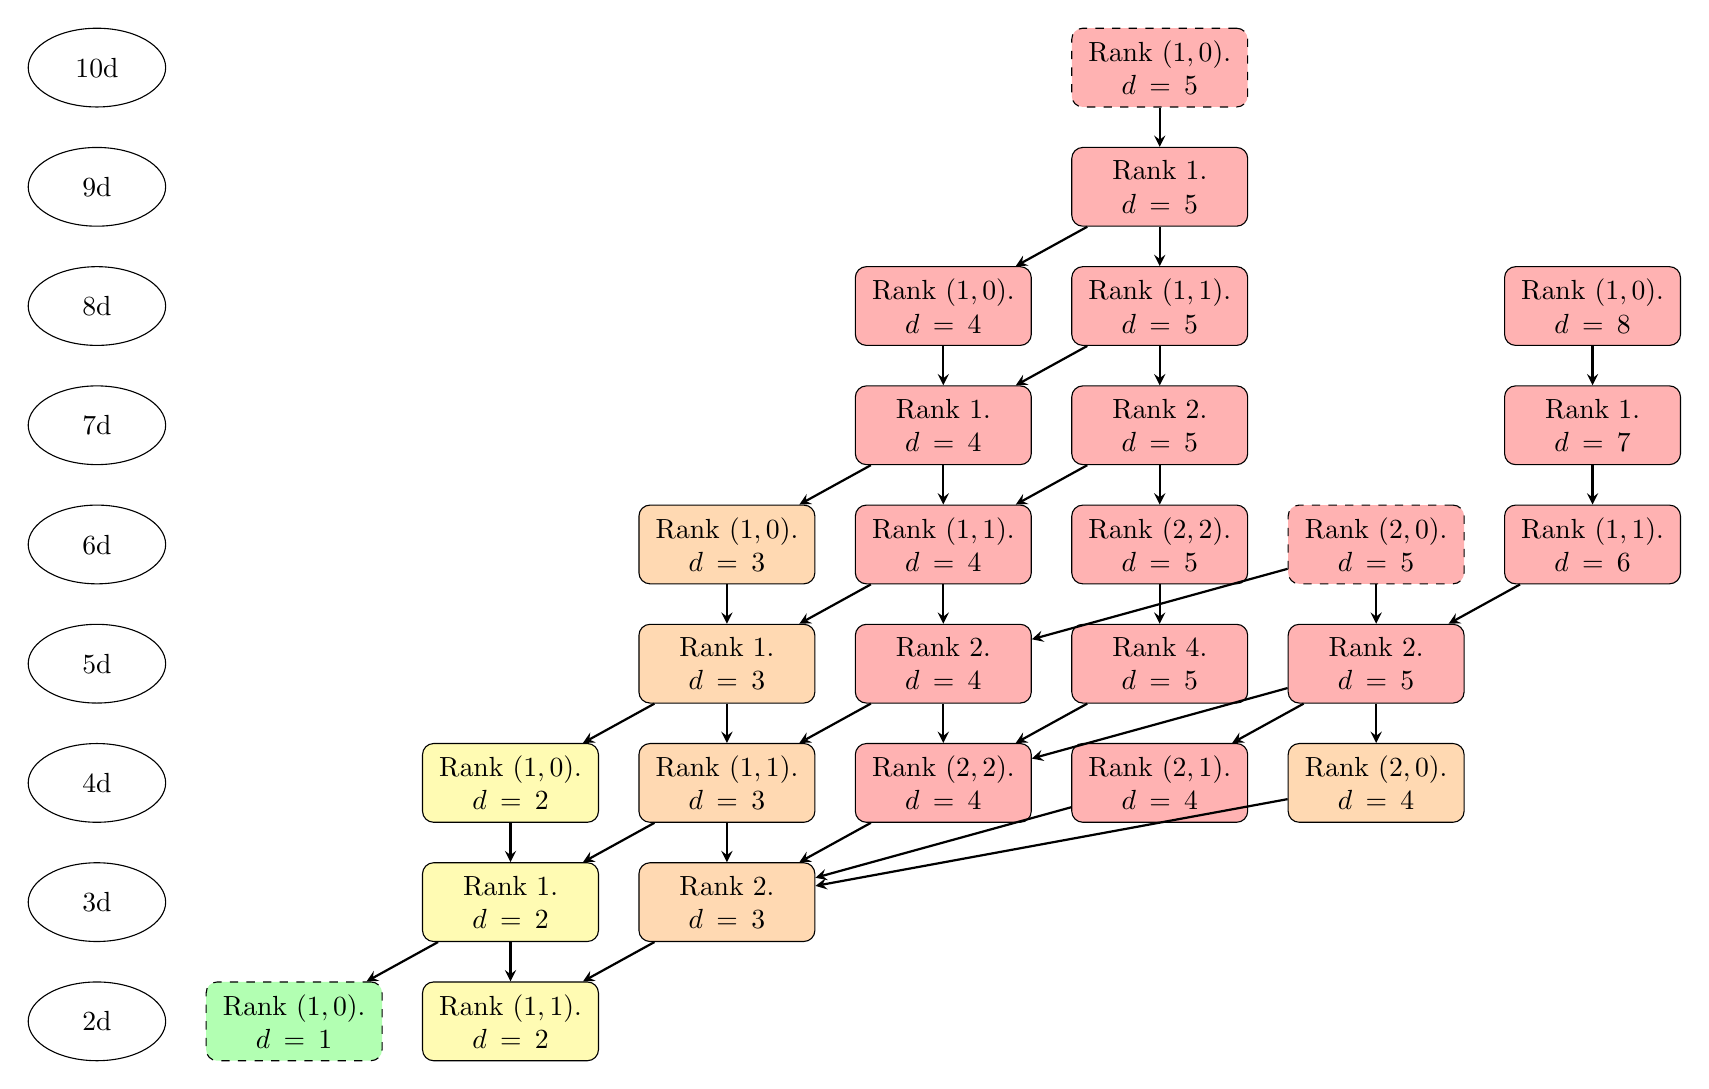
\begin{tikzpicture}[node distance=0.5cm and 0.5cm, text width=2cm]
\node (101) [s16chiral] {Rank $(1, 0)$. $d=5$};
\node (91) [s16, below=of 101] {Rank $1$. $d=5$};
\node (82) [s16, below=of 91] {Rank $(1, 1)$. $d=5$};
\node (81) [s16, left=of 82] {Rank $(1, 0)$. $d=4$};
\node (825) [right=of 82] {};
\node (83) [s16, right=of 825] {Rank $(1, 0)$. $d=8$};
\node (71) [s16, below=of 81] {Rank $1$. $d=4$};
\node (72) [s16, below=of 82] {Rank $2$. $d=5$};
\node (73) [s16, below=of 83] {Rank $1$. $d=7$};
\node (62) [s16, below=of 71] {Rank $(1, 1)$. $d=4$};
\node (61) [s8, left=of 62] {Rank $(1, 0)$. $d=3$};
\node (63) [s16, below=of 72] {Rank $(2, 2)$. $d=5$};
\node (64) [s16chiral, right=of 63] {Rank $(2, 0)$. $d=5$};
\node (65) [s16, below=of 73, right=of 64] {Rank $(1, 1)$. $d=6$};
\node (51) [s8, below=of 61] {Rank $1$. $d=3$};
\node (52) [s16, below=of 62] {Rank $2$. $d=4$};
\node (53) [s16, below=of 63] {Rank $4$. $d=5$};
\node (54) [s16, below=of 64] {Rank $2$. $d=5$};
\node (42) [s8, below=of 51] {Rank $(1, 1)$. $d=3$};
\node (41) [s4, left=of 42] {Rank $(1, 0)$. $d=2$};
\node (43) [s16, right=of 42] {Rank $(2, 2)$. $d=4$};
\node (44) [s16, right=of 43] {Rank $(2, 1)$. $d=4$};
\node (45) [s8, right=of 44] {Rank $(2, 0)$. $d=4$};
\node (31) [s4, below=of 41] {Rank $1$. $d=2$};
\node (32) [s8, below=of 42] {Rank $2$. $d=3$};
\node (22) [s4, below=of 31] {Rank $(1, 1)$. $d=2$};
\node (21) [s2chiral, left=of 22] {Rank $(1, 0)$. $d=1$};

\draw[arrow] (101) -- (91);
\draw[arrow] (91) -- (81);
\draw[arrow] (91) -- (82);
\draw[arrow] (81) -- (71);
\draw[arrow] (82) -- (71);
\draw[arrow] (82) -- (72);
\draw[arrow] (83) -- (73);
\draw[arrow] (71) -- (61);
\draw[arrow] (71) -- (62);
\draw[arrow] (72) -- (62);
\draw[arrow] (72) -- (63);
\draw[arrow] (73) -- (65);
\draw[arrow] (61) -- (51);
\draw[arrow] (62) -- (51);
\draw[arrow] (62) -- (52);
\draw[arrow] (63) -- (53);
\draw[arrow] (64) -- (52);
\draw[arrow] (64) -- (54);
\draw[arrow] (65) -- (54);
\draw[arrow] (51) -- (41);
\draw[arrow] (51) -- (42);
\draw[arrow] (52) -- (42);
\draw[arrow] (52) -- (43);
\draw[arrow] (53) -- (43);
\draw[arrow] (54) -- (43);
\draw[arrow] (54) -- (44);
\draw[arrow] (54) -- (45);
\draw[arrow] (41) -- (31);
\draw[arrow] (42) -- (31);
\draw[arrow] (42) -- (32);
\draw[arrow] (43) -- (32);
\draw[arrow] (44) -- (32);
\draw[arrow] (45) -- (32);
\draw[arrow] (31) -- (21);
\draw[arrow] (31) -- (22);
\draw[arrow] (32) -- (22);

\node (2d) [dimension, left=of 21] {2d};
\node (3d) [dimension, above=of 2d] {3d};
\node (4d) [dimension, above=of 3d] {4d};
\node (5d) [dimension, above=of 4d] {5d};
\node (6d) [dimension, above=of 5d] {6d};
\node (7d) [dimension, above=of 6d] {7d};
\node (8d) [dimension, above=of 7d] {8d};
\node (9d) [dimension, above=of 8d] {9d};
\node (10d) [dimension, above=of 9d] {10d};
\end{tikzpicture}
\caption{Orbits of square-zero supercharges.}
\label{fig:superchargeorbits}
\end{figure}
\end{landscape}

\appendix

\section{Functional analysis}

\def\CVS{{\rm CVS}}
\def\DVS{{\rm DVS}}

\brian{We can put all our conventions for topological vector spaces, largely borrowed from \cite{CG1}, here. }

\subsection{Notations and conventions}

\begin{dfn}
Let $M$ be a manifold and $E$ a (graded) vector bundle on $M$.  
For any open set $U \subset M$, define the following notations:
\begin{itemize}
\item $\cE(U)$ denotes the graded vector space of smooth sections supported on $U$;
\item $\cE_c(U)$ denotes the graded vector space of compactly supported smooth sections on $U$;
\item $\Bar{\cE}(U)$ denotes the graded vector space of distributional smooth sections on $U$;
\item $\Bar{\cE}_c(U)$ denotes the graded vector space of compactly supported distributional smooth sections on $U$.
\end{itemize}
\end{dfn}

If $E$ is a vector bundle, let $E^!$ denote the ``Verdier dual" vector bundle defined by $E^* \otimes {\rm Dens}_M$, where $E^*$ is the usual linear dual vector bundle. 
For an open set $U \subset M$ let 
\[
\cE(U)^\vee = \Bar{\cE}^!_c(U)
\]
be the continuous, or distributional dual, to $\sE(U)$. 

\begin{prop}
Let $E,F$ be vector bundles on $M,N$ respectively.
Then
\[
\cE(M) \Hat{\otimes}_\beta \cF(N) \cong \Gamma(M \times N, E \boxtimes F)
\]
\end{prop}

\begin{dfn}
Let $E$ be a vector bundle on $M$ and $U \subset M$.
The completed algebra of functions on $\cE(U)$ is
\[
\cO(\cE(U)) = \prod_{n = 0}^\infty {\rm Hom}_{\rm CVS} \left(\cE(U)^{\Hat{\otimes}_\beta n}, \CC\right)_{S_n} .
\]
\end{dfn}

\subsection{Homological algebra}

There is a functor
\[
dif_c : \CVS \to \DVS .
\]

\begin{dfn}
Suppose $V,W$ are cochain complexes in convenient vector spaces. 
A cochain map $f : V \to W$ is a {\bf quasi-isomorphism} if the map
\[
dif_c (f) : dif_c(V) \to dif_c(W)
\]
is a quasi-isomorphism of differentiable vector spaces.
\end{dfn}

\begin{dfn}
A {\bf filtered differentiable cochain complex} is a sequence of differentiable cochain complexes
\[
\cdots \to F_{n-1} V \to F_{n} V \to F_{n+1}V \to \cdots
\]
where each map is a monomorphism in each cohomological degree. 
A filtered differentiable cochain complex is {\bf complete} if the canonical maps $V \to V / F_n V$ induce an isomorphism $V \cong \lim V / F_n V$. 
\end{dfn}

\begin{thm}[Eilenberg-Moore Comparison]
Let $f : V \to W$ be a map of filtered cochain complexes in an AB4 abelian category.
Suppose, for each integer $n$ there exists an integer $p$ such that $F_p V^n = 0 = F_p W^n$.
If there is an integer $r \geq 0$ such that the induced map on the $r$th page of the corresponding spectral sequences 
\[
f_r^{pq} :  E_r^{pq} V \to E_r^{pq} W
\]
is an isomorphism for all $p,q$, then $f : V \to W$ is a quasi-isomorphism. 
\end{thm}

The category of differentiable vector space is an AB4 category, in fact, it is actually a Grothendieck abelian category. 

\begin{thm}[Theorem 2.2.1 of \cite{CG1}]
The category $\DVS$ is a Grothendieck abelian category.
\end{thm}

In particular, we can freely apply the Eilenberg-Moore comparison result to the types of topological cochain complexes we come across in the BV formalism. 

\begin{dfn}
A {\bf differentiable pro-cochain complex} is a differentiable cochain complex $V$ with a filtration
\[
\cdots \to F_{n-1} V \to F_{n} V \to F_{n+1}V \to \cdots
\]
where each map is a monomorphism in each cohomological degree and such that the canonical maps $V \to V / F_n V$ induce a quasi-isomorphism $V \to \lim V / F_n V$. 
\end{dfn}

\section{$\infty$ algebra}

\brian{Not sure if this deserves a whole appendix, but it may be good to spell out what $L_\infty$ modules are, etc..}

\end{document}
